\documentclass{article}

\usepackage{pgf}
\usepackage{tikz}
\usetikzlibrary{arrows,automata,decorations.pathmorphing,backgrounds,positioning,fit,petri}

\begin{document}

\section{Bachelorarbeit}

\subsection{Initial formulation of the problem}

\subsubsection{Open questions and degress of freedom}

\begin{enumerate}
  \item How to set the maximum thresholds of the network: in the Thomas
  framework, the maximum threshold is given by the number of outgoing edges, but
  one could introduce multiple edges in order to increase the impact of a
  predecessor on a successor node. This question might be investigated
  systematically.
  \item How to set the edge labels of the network: e.g. is an activating node
  {\tt +} or just {\tt obs+} or even another edge label? Again, this question
  might be investigated systematically.
  \item How to exactly define a stripe? This question must be investigated
  systematically, both in terms of CTL and in terms of AL.
  \item Furthermore, the intersection of the CTL and AL parameter sets must be
  investigated. Are the same parameter sets filtered by AL and CTL? I.e., is a
  stripe under CTL the same as a stripe in AL? If not, is one approach more
  comprehensive than the other?
\end{enumerate}

Note: for the stripe, we need at least three different values for the morphogene
(high, medium, low). Hence we need to artificially introduce those---either by
multi-edges or by more than one formal morphogene. E.g. two formal, identical
morphogenes are able to produce three different states of activity: both
inactive (low), one active (medium), both active (high).

\subsubsection{From simple to complicated - a research program}

\begin{enumerate}
  \item We will investigate one particular network with only 3 nodes (4 or 5
  with morphogene).
  \item We will apply the strictest possible edge labels ({\tt +} and {\tt -}
  initially).
  \item The dynamics are to be investigated in particular using Cytoscape.
  \item We will try out all possible values for thresholds and record the
  results for each set.
  \item Results are to be recorded for CTL filtering, for AL filtering and for
  the combination of CTL filtering and AL filtering.
  \item Next the edge label strictness can be relaxed. Again, all results are to
  be recorded.
  \item Afterwards, this procedure is to be applied for all simple
  stripe-generating networks with three nodes (diffusion to be left out initially).
  \item Finally, networks with more nodes can be investigated.
\end{enumerate}

\subsubsection{Defining stripes}

in CTL

in AL

\subsection{Other To Dos}

\begin{enumerate}
  \item Describe the connection between the quasi-continous formalism and the
  Thomas formalism
  \item Enumerate all possible (connected) networks in Python
\end{enumerate}

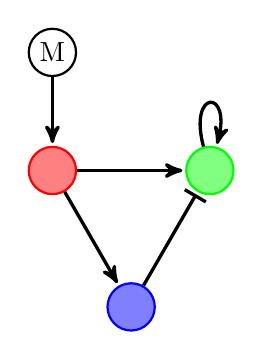
\begin{tikzpicture}
[->,>=stealth',shorten >=1pt,
gene/.style={circle,thick,inner sep=0pt,minimum size=6mm}]
\node[gene,draw=black,fill=white]    at (90:1.5cm)  (mm) {M};
\node[gene,draw=red,fill=red!50]     at (0,0)     (rr) {};
\node[gene,draw=blue,fill=blue!50]   at (300:2cm) (bb) {};
\node[gene,draw=green,fill=green!50] at (0:2cm)   (gg) {};

\path [->,very thick] (mm) edge node {} (rr);
\path [->,very thick] (rr) edge node {} (gg);
\path [->,very thick] (rr) edge node {} (bb);
\path [-|,very thick] (bb) edge node {} (gg);
\path [->,very thick] (gg) edge [loop above,looseness=12] node {} (gg);
\end{tikzpicture}

\end{document}
